%% Template for a preprint Letter or Article for submission
%% to the journal Nature.
%% Written by Peter Czoschke, 26 February 2004
%%

\documentclass[extra,mreferee]{gji}
\usepackage{graphicx}
\usepackage[labelformat=empty]{caption}
%% make sure you have the nature.cls and naturemag.bst files where
%% LaTeX can find them

%\bibliographystyle{naturemag}

\title{Supporting Information for \\ ``Controls on Surface Wave Overtone Interference"}

\author[Hariharan et al.]
  {Anant Hariharan$^1$, Colleen A. Dalton$^1$,  Jordyn Babikoff$^1$, G{\"o}ran Ekstr{\"o}m$^2$ \\
  $^1$ Department of Earth, Environmental, and Planetary Sciences, Brown University, Providence, RI, United States\\
  $^2$ Lamont-Doherty Earth Observatory of Columbia University, United States}

\begin{document}

\maketitle



\noindent\textbf{Contents of this file}
%%%Remove or add items as needed%%%
\begin{enumerate}
%\item Text S1 to Sx
\item Figures S1 to S10
%\item Tables S1 to Sx
%if Tables are larger than 1 page, upload as separate excel file
\end{enumerate}
%\noindent\textbf{Additional Supporting Information (Files uploaded separately)}
%\begin{enumerate}
%\item Captions for Datasets S1 to Sx
%\item Captions for large Tables S1 to Sx (if larger than 1 page, upload as separate excel file)
%\item Captions for Movies S1 to Sx
%\item Captions for Audio S1 to Sx
%\end{enumerate}

%\noindent\textbf{Introduction}
%This document contains supplementary figures S1-10.
\newpage
\begin{figure}
 \noindent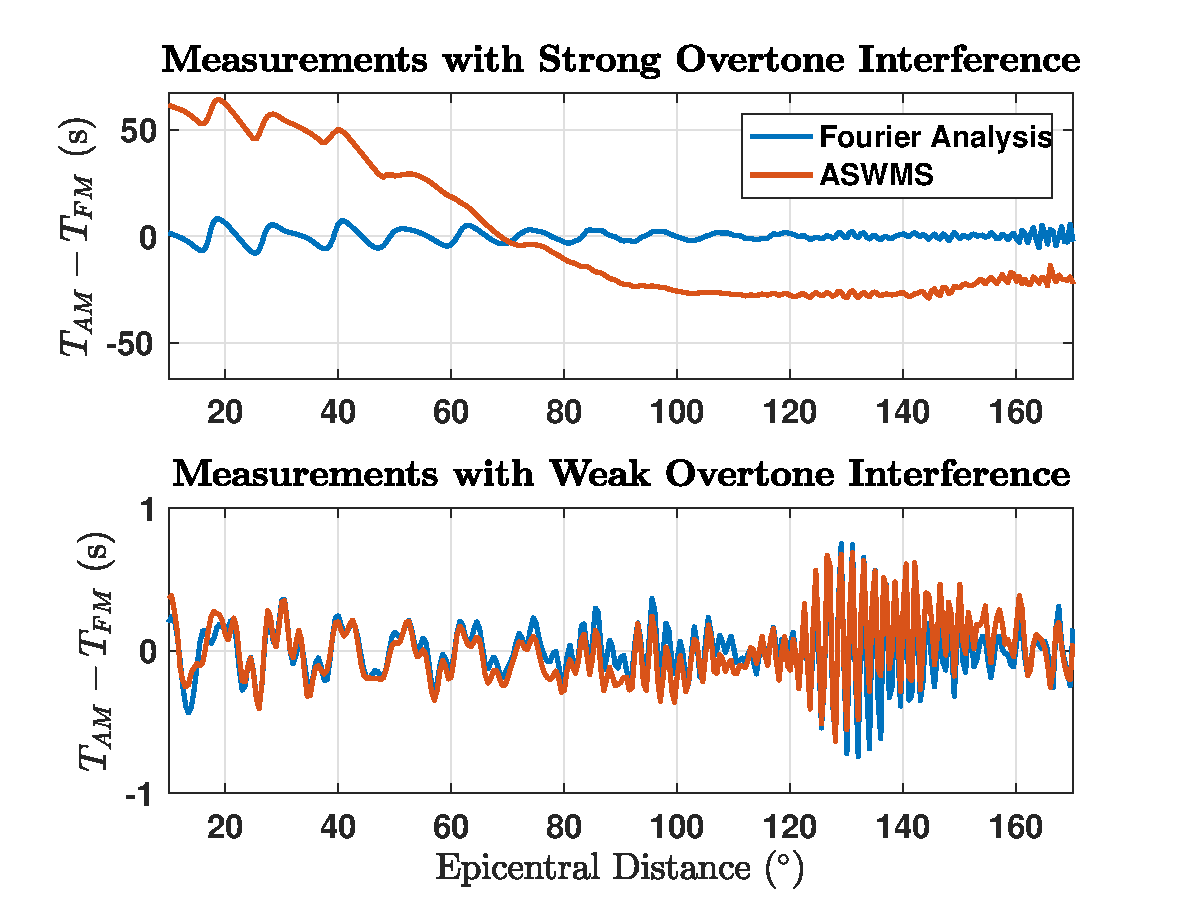
\includegraphics[width=1\textwidth]{FigS1_VSver.eps} \end{figure} \textbf{Figure S1}: Travel-time interference pattern, for 100-s Rayleigh waves, for an event with strong overtone interference (top) and weak overtone interference (bottom). The measurements have been repeated for two approaches: using ASWMS (orange) and Fourier analysis (blue). Note the different vertical scales.

\newpage
\begin{figure}
 \noindent\includegraphics[width=1\textwidth]
{FigS2_VSver.eps} \end{figure} 
\textbf{Figure S2}: Love wave excitation as a function of depth for the FM and first overtone. (a-c): Calculations for ATL2a. (d-f): Calculations for STW105-C. Each column is a different end-member source mechanism. Dashed line: fundamental mode. Solid line: first overtone.


\newpage
\begin{figure}
 \noindent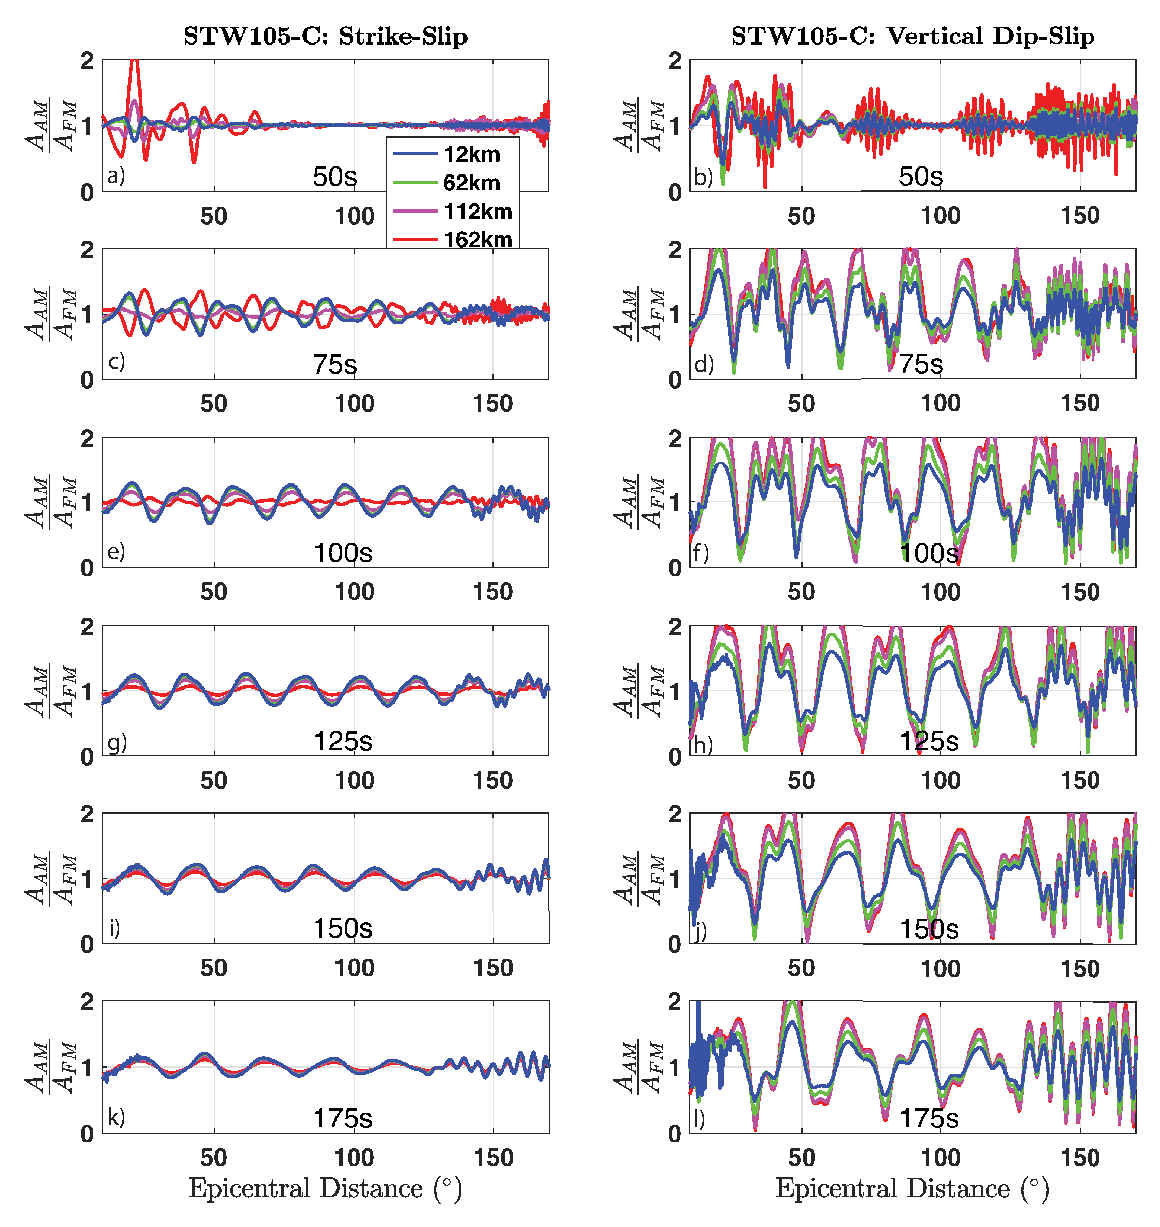
\includegraphics[width=1\textwidth]{FigS3_VSver.eps}
\end{figure}
\textbf{Figure S3}: Plots of the Love wave amplitude interference pattern, color-coded by source depth, for end-member source geometries (as in Fig.4 in the main text) and for the continental Earth model STW105-C. Left column: Interference patterns for a strike-slip event. Right column: Interference patterns for a vertical dip-slip event.  

\newpage
\begin{figure}
 \noindent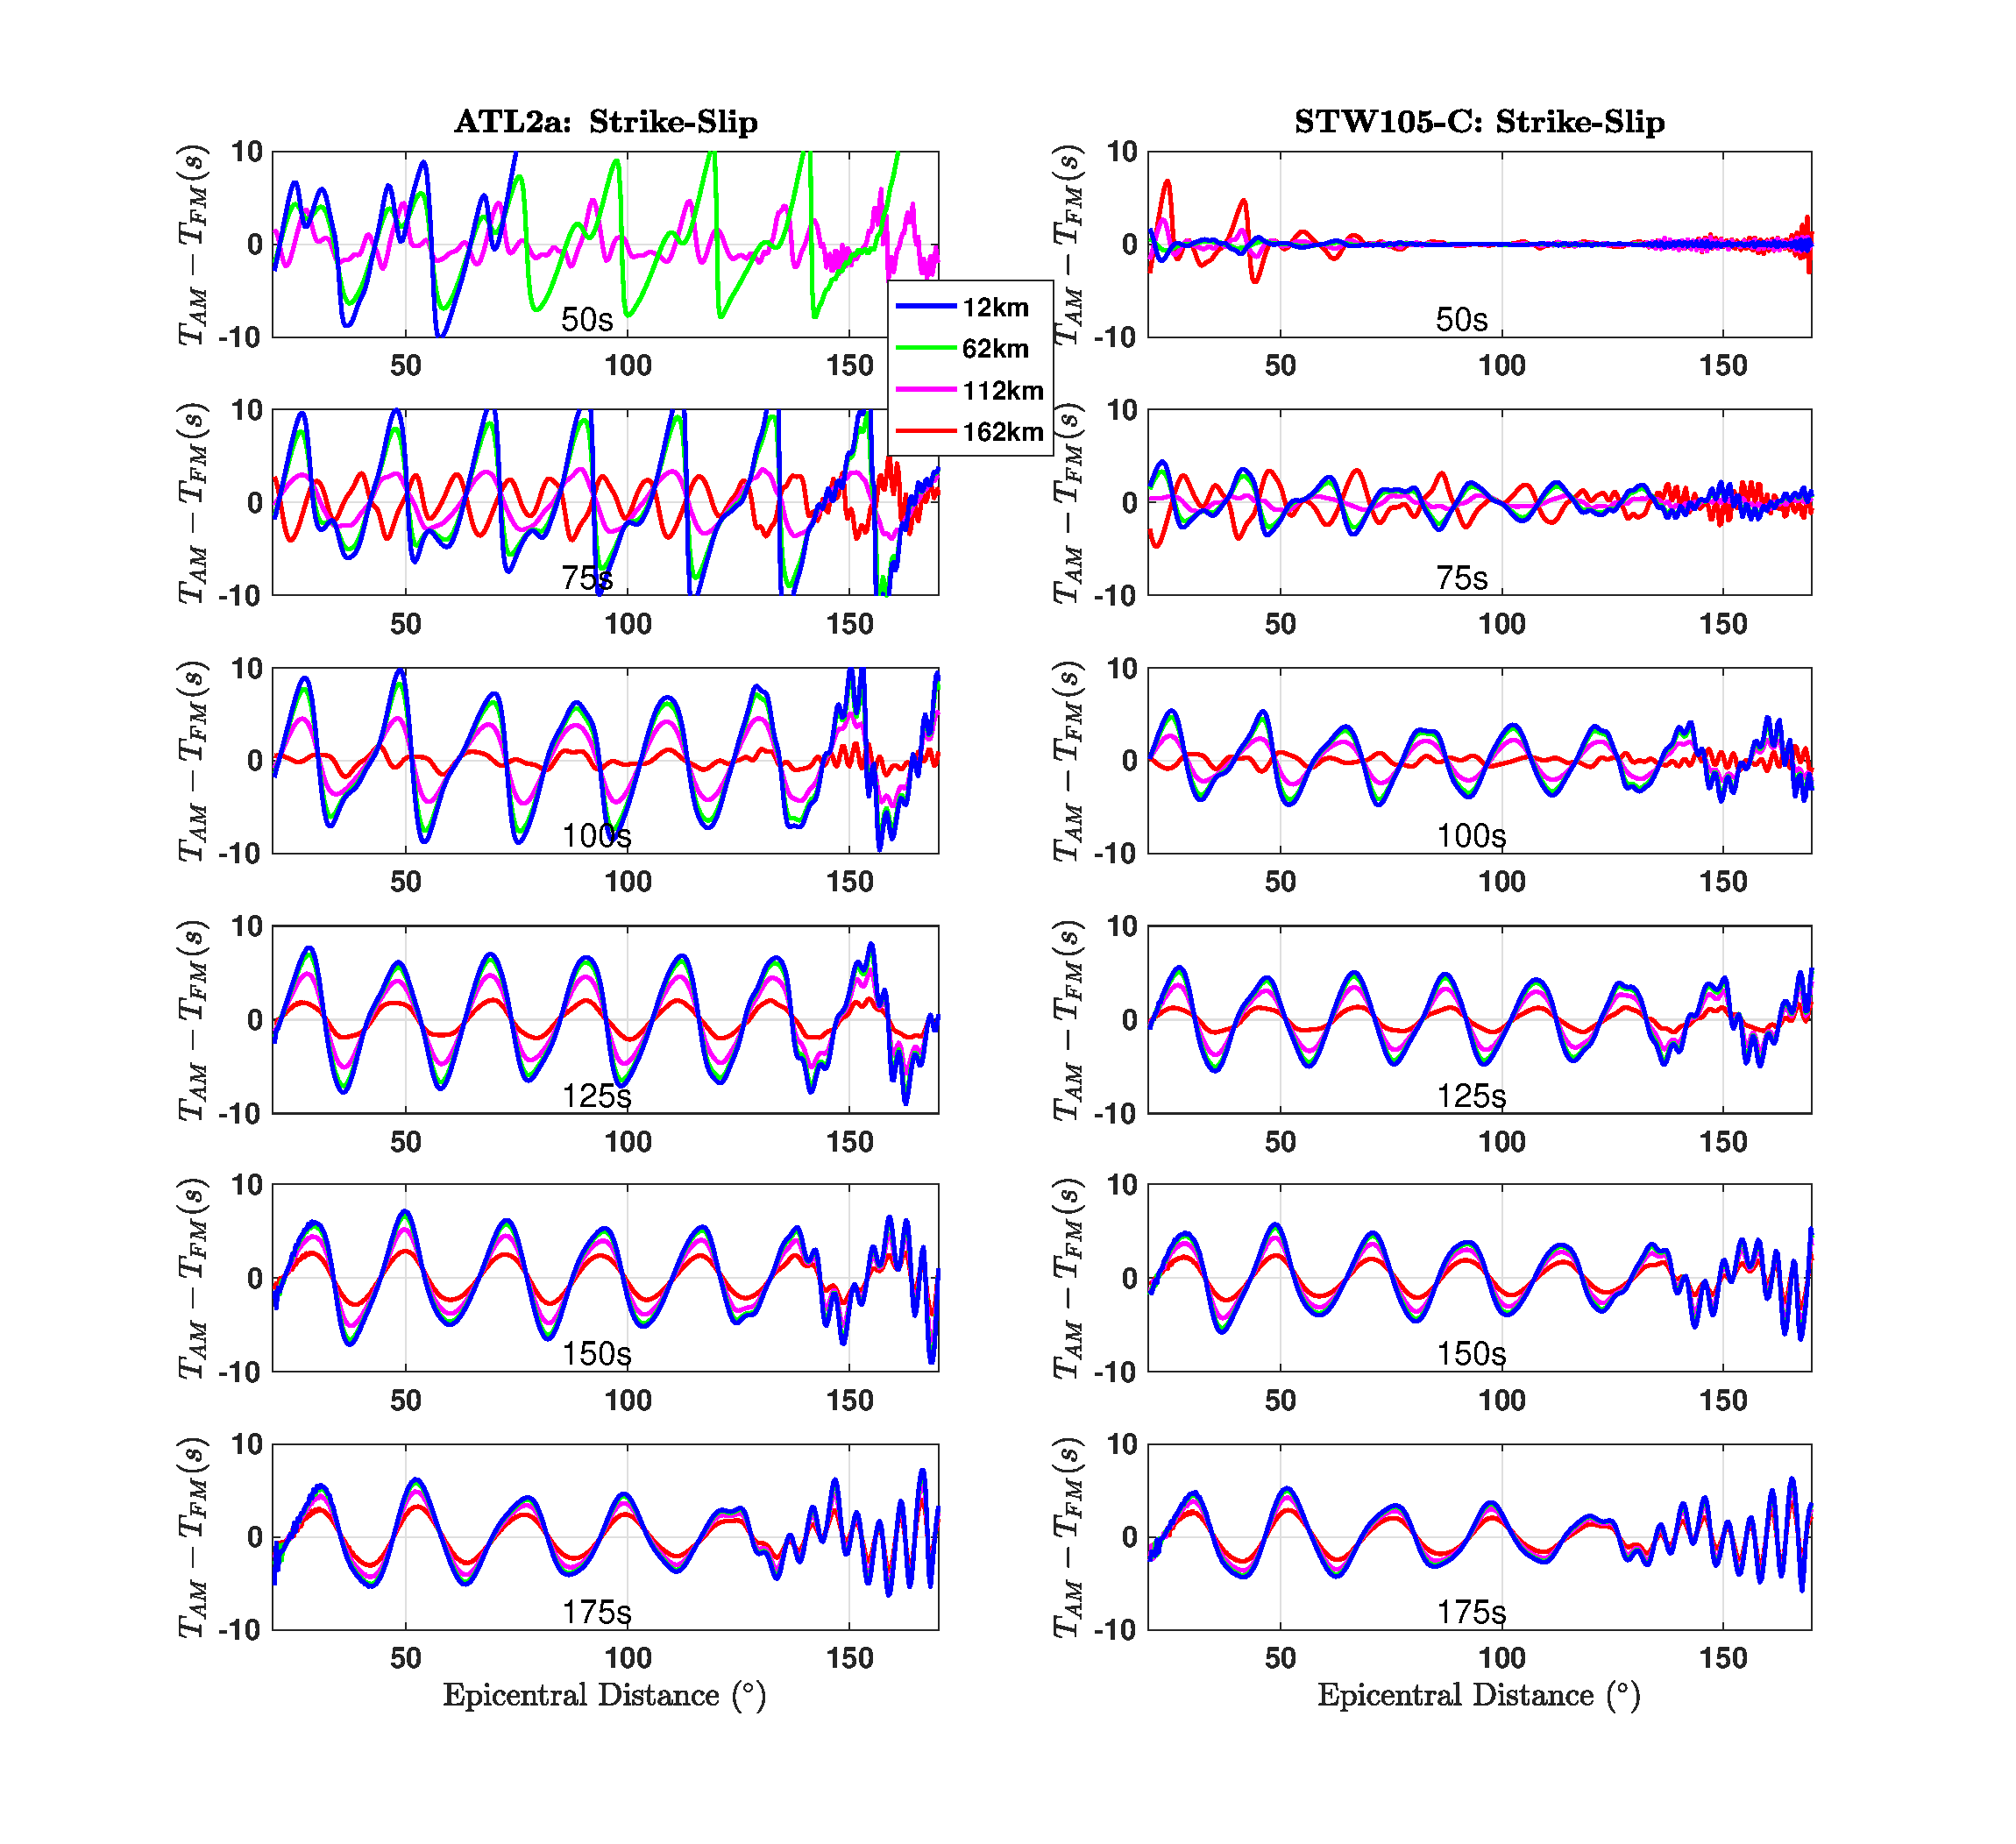
\includegraphics[width=1\textwidth]{FigS4_VSver.eps}
\end{figure}
\textbf{Figure S4}: Love wave traveltime interference patterns at different periods, color-coded by source depth, for a strike-slip source. Left: Measurements for ATL2a. Right: measurements for STW105-C.

\newpage
\begin{figure}
 \noindent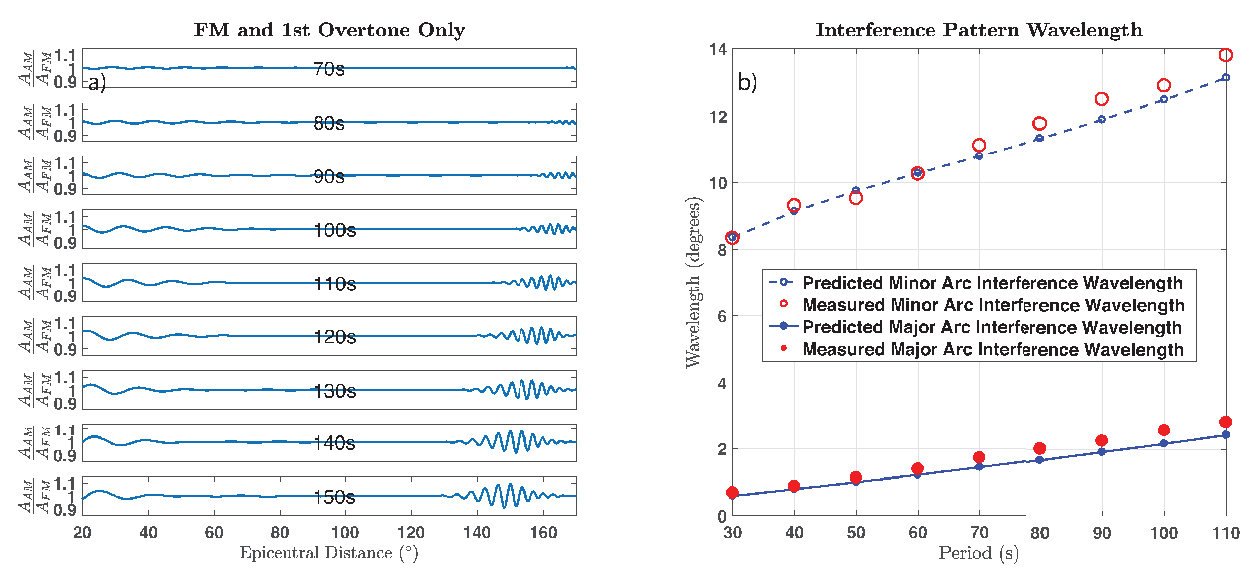
\includegraphics[width=1\textwidth]{FigS5_VSver.eps}
\end{figure}
\textbf{Figure S5}: (a) Amplitude interference patterns determined from normal-mode synthetic seismograms with an explosive source. The vertical axis shows the ratio of amplitudes measured from synthetic seismograms that contain the first and fundamental modes to those measured from synthetic seismograms containing only the fundamental mode. (b) Comparison of interference wavelength measured from the amplitude interference patterns (see text) to that predicted using Equations 3 and 4.

\newpage
\begin{figure}
 \noindent\includegraphics[width=1\textwidth]{FigS6_VSver.eps}
\end{figure}
\textbf{Figure S6}: Rayleigh wave amplitude interference patterns across both the distance range prone to minor-arc overtone interference and that prone to major-arc overtone interference, color-coded by depth and shown at all periods analyzed. Each column corresponds to a different end-member source mechanism.

\newpage
\begin{figure}
 \noindent\includegraphics[width=1\textwidth]{FigS7_VSver.eps}
\end{figure}
\textbf{Figure S7}: As in figure S6, but showing Rayleigh wave travel time interference patterns instead of amplitude interference patterns. The measurements that go off-scale are (1) The 62-km deep Strike-Slip event measured at 75s, (2) The 62-km deep Strike-Slip event measured at 100s, (3) The 62-km deep 45$^\circ$ Dip-Slip event measured at 100s, (4) The 62-km deep 45$^\circ$ Dip-Slip event measured at 125s, (5) The 112-km deep Strike-Slip event measured at 150s, (6) The 112-km deep Strike-Slip event measured at 175s. 

\newpage
\begin{figure}
 \noindent\includegraphics[width=1\textwidth]{FigS8_VSver.eps}
\end{figure}
\textbf{Figure S8}: As in figure 10, but showing traveltime interference patterns instead of amplitude interference patterns: Interference patterns color-coded by depth for Rayleigh (left) and Love (right) waves across a range of periods. The interference patterns are computed for 200 randomly selected events from the Global CMT catalog with source depth between 15 and 50 km.

\newpage
\begin{figure}
\noindent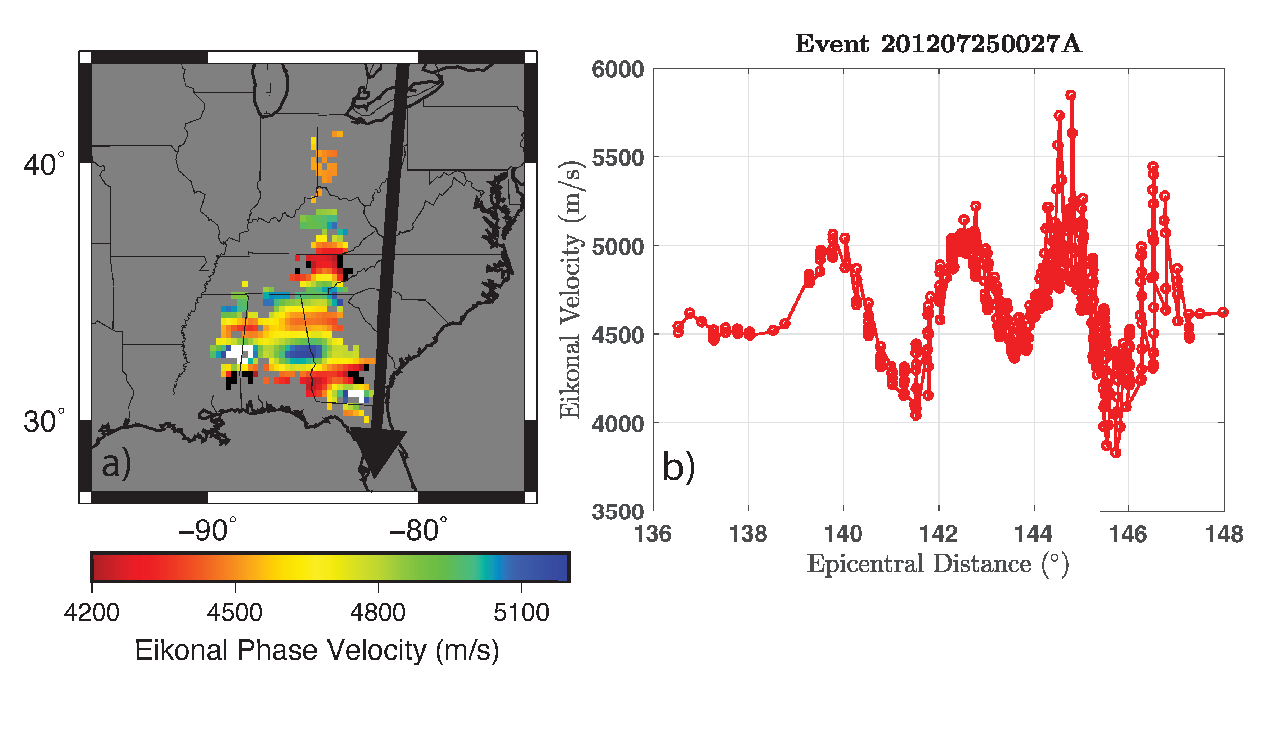
\includegraphics[width=0.98\textwidth]{FigS9_VSver.eps}
\end{figure}
\textbf{Figure S9}: Example of Love wave major-arc overtone interference at 75 s. (a) Eikonal velocities in map view. (b) Eikonal velocities plotted as a function of epicentral distance. Measurements are made using phase-matched filtering on event ID 201207250027A, which is located at 95.93$^\circ$E, 2.46$^\circ$N, and at a depth of 20 km. The black arrow illustrates a great-circle ray path.


\newpage
\begin{figure}
 \noindent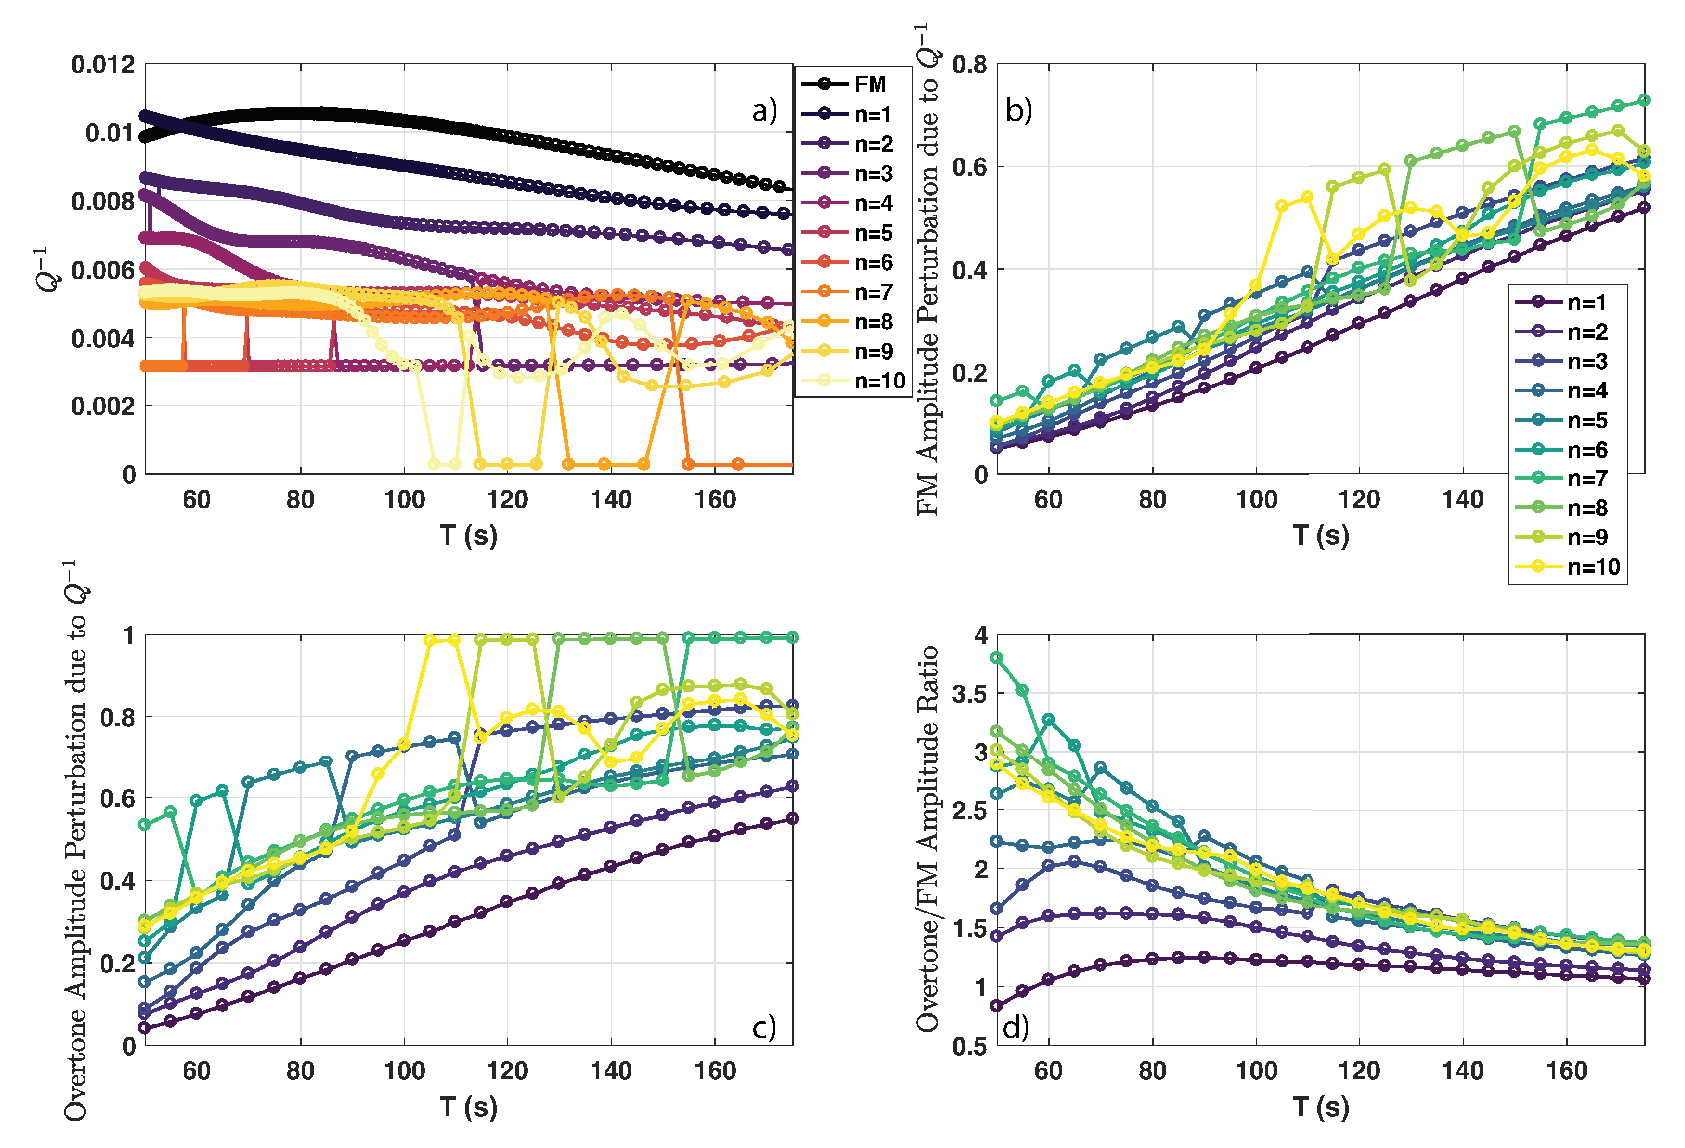
\includegraphics[width=1\textwidth]{FigS10_VSver.eps}
\end{figure}
\textbf{Figure S10}: The impact of attenuation on Rayleigh wave major-arc interference. a) Rayleigh wave attenuation ($Q^{-1}$) as a function of period for the first 10 overtones and FM. b)  Amplitude perturbation to the FM at the distance at which it intersects an overtone, due to attenuation. c) Amplitude perturbation to the overtone at the distance at which it intersects the FM, due to attenuation. d) Ratio of the amplitude calculations in (c) and (b).

\newpage
\begin{figure}
 \noindent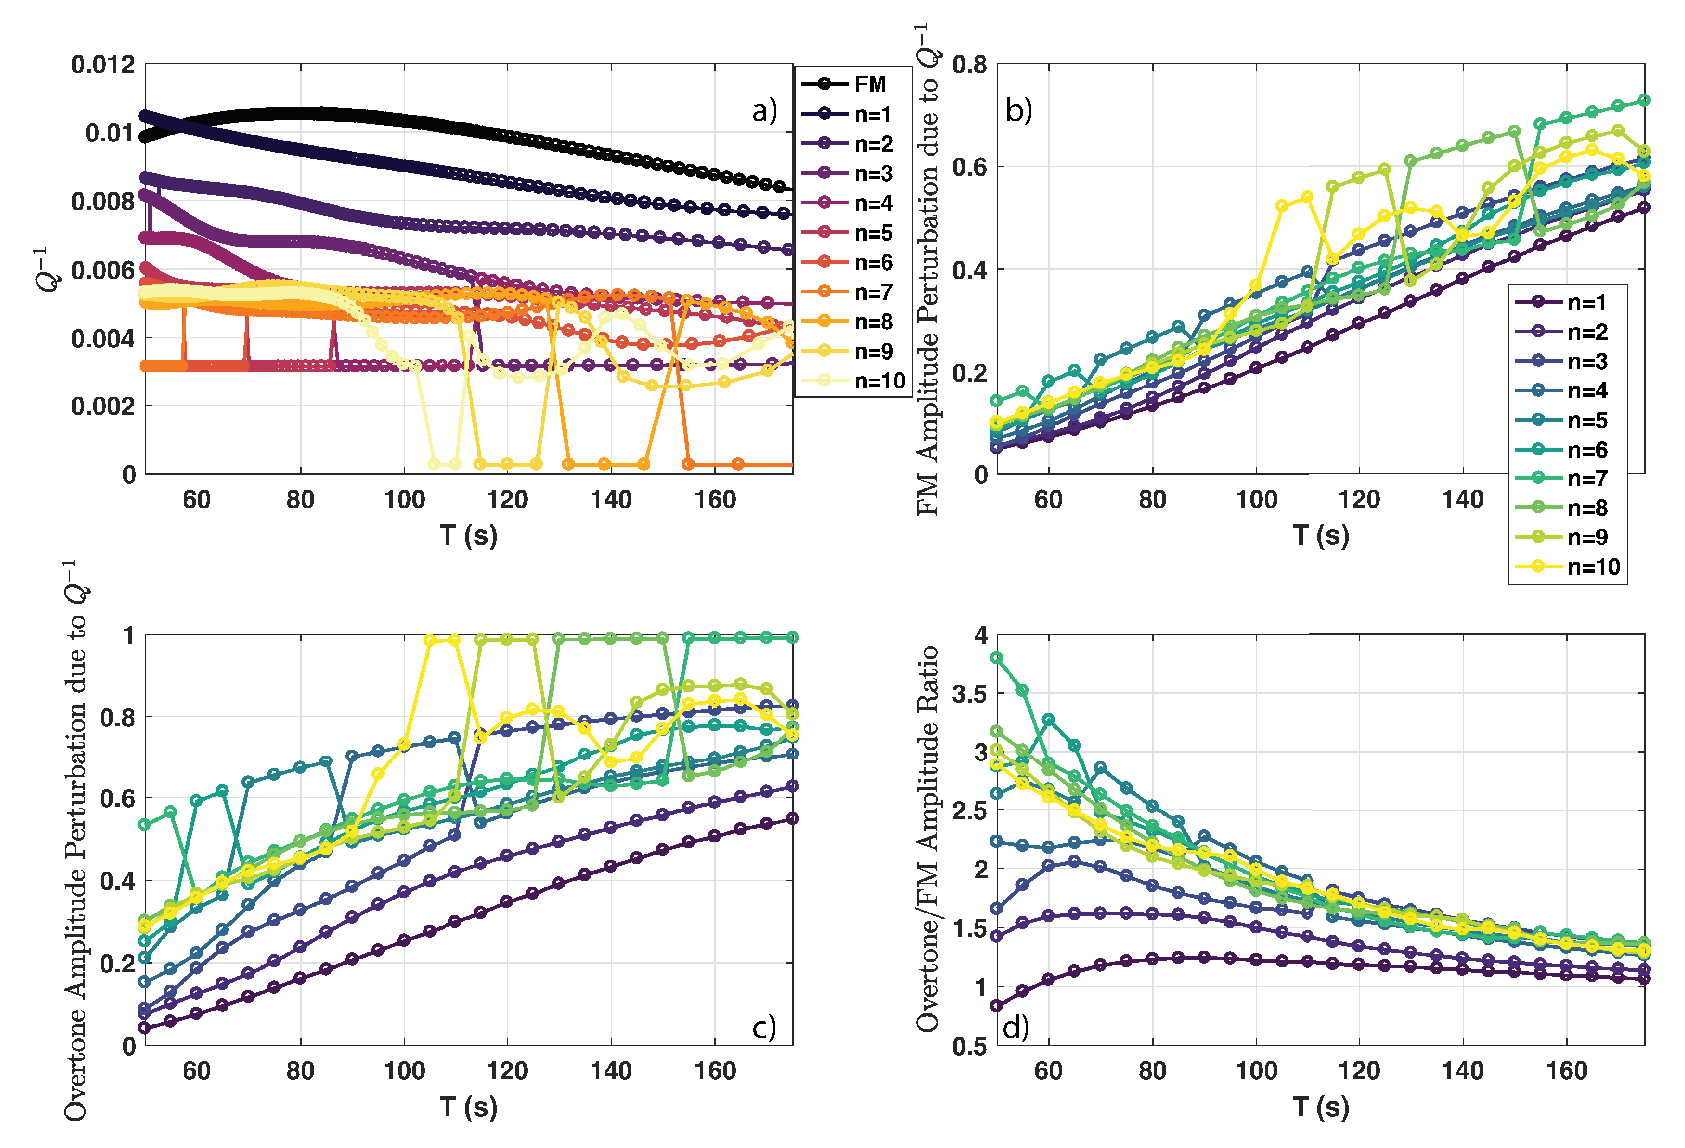
\includegraphics[width=1\textwidth]{FigS10_VSver.eps}
\end{figure}
\textbf{Figure S11}: As in the left y-axis in Figure 14c), but for both Eikonal (red) and Helmholtz (blue) phase velocities. Error in phase velocity measurements, relative to the GDM52 phase velocity maps, is binned as a function of epicentral distance. Measurements are for Rayleigh waves at 100s. 

%% Put the bibliography here, most people will use BiBTeX in
%% which case the environment below should be replaced with
%% the \bibliography{} command.



%% Here is the endmatter stuff: Supplementary Info, etc.
%% Use \item's to separate, default label is "Acknowledgements"



%%
%% TABLES
%%
%% If there are any tables, put them here.
%%
\newpage
\newpage
%\begin{thebibliography}{1}
%\bibitem{dummy} Articles are restricted to 50 references, Letters
%\bibitem{dummyb} No compound references -- only one source per
%\end{thebibliography}

\end{document}